\subsection{Không gian vector}
\subsubsection*{Cơ sở}
Trong phần vừa rồi, khi giới thiệu về khái niệm vector cơ sở, chúng được giới thiệu là một hệ vector trực chuẩn, tức là lẫn nhau vuông góc (có tích vô hướng bằng \(0\)) và có độ dài bằng \(1\).
Nhưng điều này không hề tổng quát, hay cụ thể hơn, một hệ vector cơ sở có thể hoặc là hoặc không là một hệ vector trực chuẩn, và có thể có vô số hệ cơ sở trong không gian. 
\vspace{5pt}

Dựa theo định nghĩa, một hệ vector cơ sở là hệ vector sao cho mọi vector trong không gian đều có thể được phân tích thành một \emph{tổ hợp tuyến tính} của chúng. Nói cách khác, giả sử ta có hai vector cơ sở \(\mathbf{e}_i\) và \(\mathbf{e}_j\), một vector \(\mathbf{v}\) bất kỳ có thể được viết thành \[\mathbf{v}=\alpha\mathbf{e}_1 +\beta\mathbf{e}_2,\] với \[\alpha,~\beta \quad \in\mathbb{R}.\] Ta lại xét một hệ cơ sở khác gồm hai vector \(\mathbf{e}_{3}, \mathbf{e}_4\), lúc này \[\mathbf{v}=\gamma\mathbf{e}_3 +\sigma\mathbf{e}_4.\]
Ví dụ sau đây sẽ làm sáng rõ nội dung vừa rồi: 
\[\mathbf{v}= (5;3)=5(1;0)+3(0;1)=1(2;-3)
+3(1;2).\] Vector \(\mathbf{v}\) đầu tiên được phân tích thành hai vector cơ sở ta đã quen thuộc, rồi sau đó lại được phân tích thành hai vector \[
\mathbf{e}_3 =(2;-3),\qquad \text{ và } \mathbf{e}_4 =(1;2).\] 
\begin{figure}[H]
    \centering
    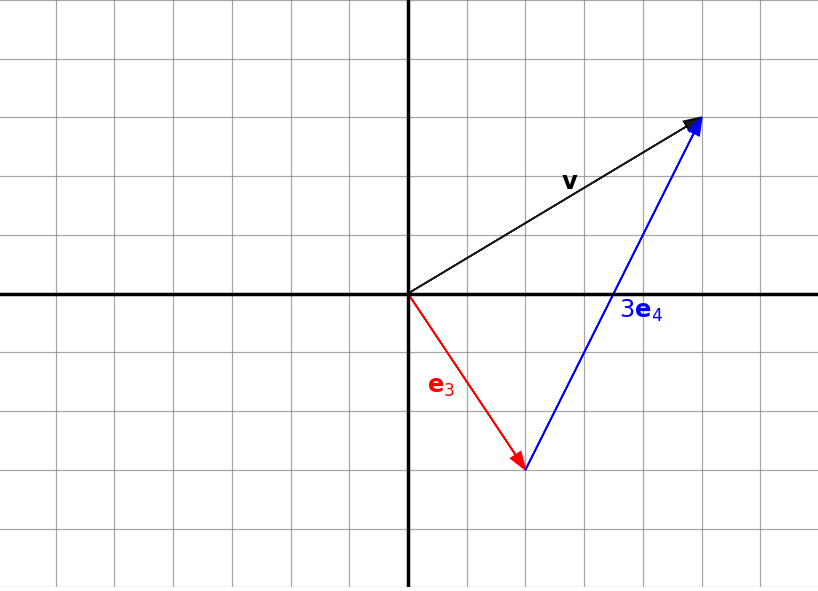
\includegraphics[width=0.8\linewidth]{Tuan1/ảnh/e3e4.png}
\end{figure}
Dễ thấy, hai vector này không trực giao, cũng không có độ lớn bằng \(1\). 

Một tổ hợp tuyến tính của hai vector nói rằng ta đã kéo giãn mỗi vector theo một hệ số nào đó và sau đó cộng chúng với nhau. Đặc biệt, đối với hai vector mới được chọn, bằng cách lựa chọn một bộ hệ số vô hướng thích hợp, ta có thể biểu diễn mọi vector trên mặt phẳng thành một tổ hợp tuyến tính của chúng (do đó ta chọn chúng làm cơ sở, như đã đề cập). 
Mặt khác, nếu hai vector ta chọn chỉ là \(\mathbf{e}_3\) và, chẳng hạn, \(2\mathbf{e}_3\), những vector có thể được biểu diễn bởi hệ cơ sở này chỉ có những vector nằm trên cùng một đường thẳng với \(\mathbf{e}_3\). Nhưng đồng thời, nếu ta chỉ quan tâm tới 
những thứ xảy ra trên đường thẳng đó, thì bất kỳ một vector nào nằm trên đó đều là cơ sở cho \emph{không gian}(đường thẳng) mà ta quan tâm.
\vspace{8pt}

Một cách tự nhiên, ta đi tới những khái niệm sau:
\begin{definition}[Bao tuyến tính]
    Nếu \(S={\mathbf{u}_{1}, \mathbf{u}_{2},\dots,  \mathbf{u}_{n}}\) là một tập hợp \(n\) vector trong không gian, thì tập hợp tất cả các tổ hợp tuyến tính của chúng được gọi là bao tuyến tính của \(\mathbf{u}_{1}, \mathbf{u}_{2},\dots \mathbf{u}_{n}\), và được kí hiệu là span(\(S\)).
    \vspace{8pt}

    Nếu span(S) chứa toàn bộ vector trong không gian, vậy ta gọi S là một hệ sinh cho không gian.
\end{definition}

\begin{definition}[Độc lập tuyến tính]
    Một tập hợp các vector được gọi là \emph{độc lập tuyến tính} với nhau nếu tổ hợp tuyến tính của chúng không bao giờ bằng \(\mathbf{0}\) trừ khi \textbf{tất cả} các hệ số vô hướng đều bằng \(0\).
\end{definition}
\begin{definition}[Hệ cơ sở]
    Một cơ sở của không gian là một tập hợp các vector trong không gian sao cho 
    \begin{itemize}
        \item tạo thành hệ sinh cho không gian, và
        \item độc lập tuyến tính.\footnote{Có thể chứng minh rằng mỗi vector trong không gian tương ứng với duy nhất một tổ hợp tuyến tính của cùng một hệ cơ sở. Đây là một bài tập cho các bạn.}
    \end{itemize}
\end{definition}
Trong ví dụ cụ thể ta đã lấy ở trên, không gian của ta (một mặt phẳng) có hai hệ sinh là \(S_1 ={\mathbf{e}_{1}, \mathbf{e}_2}\), và \(S_2 ={\mathbf{e}_{3}, \mathbf{e}_{4}}\). Đồng thời, hai cặp vector tạo thành hai hệ sinh này cũng là các cơ sở khác nhau. Ngoài ra cũng chú ý rằng, \(S_{3}={\mathbf{e}_{3}, \mathbf{e}_{4}, 2\mathbf{e}_{3}}\) cũng là một hệ sinh cho mặt phẳng này nhưng tập hợp ba vector này không phải là một hệ cơ sở, vì nó không độc lập tuyến tính (phụ thuộc tuyến tính). Cụ thể, dễ thấy rằng \[-2\mathbf{e}_{3}+1(2\mathbf{e}_{3})+0\mathbf{e}_{4}=\mathbf{0},\] nhưng ta lại có các hệ số khác \(0\) là \(-2\) và \(1\).

\subsubsection*{Không gian vector}
Khi đề cập đến vector, ta không tránh khỏi đề cập đến từ "không gian". Trong phần \ref{vector}, từ này được hiểu là không gian ba chiều mà ta sinh hoạt, có trên dưới, phải trái, trước sau; tức là không gian hình học. Song, trong phần vừa rồi, từ "không gian" được dùng một cách nhập nhằng, tối nghĩa. Thoạt đầu là nghĩa ở \ref{vector}. Rồi trong các phần định nghĩa mới được đưa ra, nó dường như cũng chỉ để chỉ mặt phẳng toạ độ Oxy, chỉ chứa các vector có hai thành phần toạ độ. Số vector cơ sở cho không gian này cũng chỉ là \(2\) mà không phải \(3\). Việc nói rằng "bởi vì vector đại diện cho trên dưới lúc này bằng \(\mathbf{0}\) nên không được xét vào" là vô nghĩa và không đúng với các định nghĩa được đưa ra. 
Thành thử, cần làm rõ nghĩa của cụm "không gian chứa các vector".
\vspace{8pt}

\begin{definition}\label{def2.2.4}
    Một không gian vector \(V\) là một tập hợp mà các phần tử trong đó, được gọi là vector thoả mãn 
    \begin{enumerate}
        \item[(i)] Với mọi \(\mathbf{v}, \mathbf{w}\in V , \mathbf{v}+\mathbf{w}\in V\).
        \item[(ii)] Với mọi \(\mathbf{v}\in V, \alpha\in \mathbb{R}, \alpha\mathbf{v}\in V\).
        \item[(iii)]  \(\mathbf{v}+\mathbf{w}=\mathbf{w}+\mathbf{v}\).
        \item[(iv)]    \(\mathbf{u}+(\mathbf{v}+\mathbf{w})=(\mathbf{u}+\mathbf{v})+\mathbf{w}\).
    \end{enumerate}
\end{definition}
Dưới góc nhìn của một tập hợp, ta quay lại với ba ví dụ quen thuộc cho không gian vector:
\begin{enumerate}[label=(\alph*)]
    \item Trục số thực: \(\mathbb{R}^1\)
    \begin{figure}[H]
        \centering
        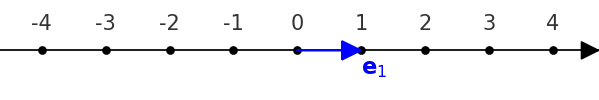
\includegraphics[width=0.8\linewidth]{Tuan1/ảnh/realaxis.png}
    \end{figure}
    Rõ ràng, tập hợp các số thực \(\mathbb{R}\) cũng là một không gian vector với duy nhất một vector cơ sở là \(1\) (hoặc bất kỳ số thực nào khác). Mỗi vector có thể được biểu diễn bằng một toạ độ -một điểm trên trục số, và từ đó là toàn bộ hệ sinh.
    \item Mặt phẳng toạ độ: \(\mathbb{R}^2\)
    \begin{figure}[H]
        \centering
        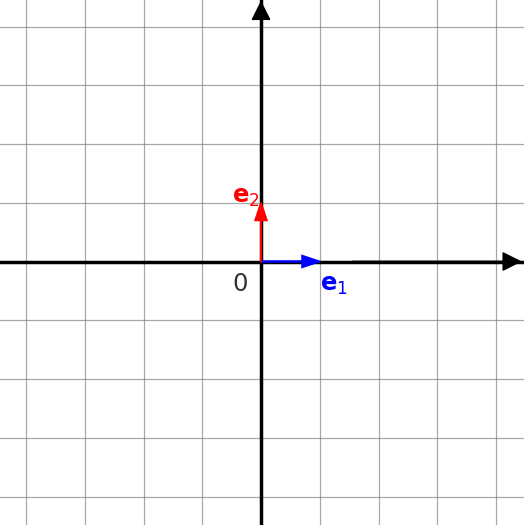
\includegraphics[width=0.6\linewidth]{Tuan1/ảnh/2Dvectorspace.png}
    \end{figure}
    Với không gian vector quen thuộc này, ta kí hiệu nó là \(\mathbb{R}^2\). Hai cơ sở quen thuộc là \((1;0)\) và \((0;1)\), với mỗi vector được biểu diễn bằng hai toạ độ, và do đó là một nút của hai đường thẳng vuông góc với trục tung, trục hoành. Rồi từ đó là toàn bộ hệ sinh.
    \item Không gian hình học: \(\mathbb{R}^3\)
    \begin{figure}[H]
        \centering
        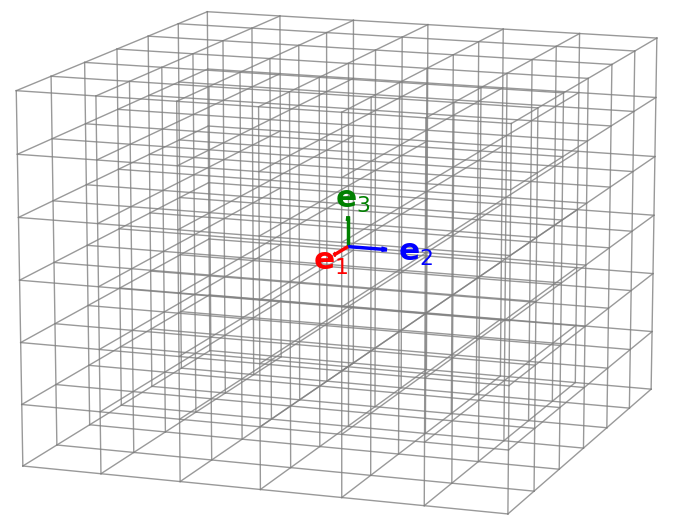
\includegraphics[width=0.6\linewidth]{Tuan1/ảnh/3Dvectorspace.png}
    \end{figure}
    Với trường hợp này, ta cần ba vector cơ sở và tương ứng là ba toạ độ cho mỗi vector. Hệ sinh của không gian được minh hoạ như trong hình.
\end{enumerate}
Nhận thấy rằng các trường hợp trên khác nhau bởi số lượng của vector cơ sở\footnote{Có thể chứng minh rằng số lượng vector cơ sở cho cùng một không gian là duy nhẩt. Xem \emph{Chapter 3. Introduction to Linear Algebra. Gilbert Strange. 5th} cho một chứng minh với các vector thực.}, khái niệm \emph{chiều} của một không gian vector vì vậy dược định nghĩa là số lượng của các vector cơ sở trong hệ cơ sở của không gian đó. Các trường hợp có chiều là \(1,2,3\) đã được đề cập. Vậy \(4,5,\dots n\) thì sao? Ta không thể minh hoạ được các ví dụ này, nhưng có thể biểu diễn các vector trong, không gian vector \(\mathbb{R}^4\) bằng một vector có bốn toạ độ là, chẳng hạn, \((1,2,3,3)\), tức là một mảng số một chiều có bốn thành phần. Tương tự, \(n\) toạ độ cho \(\mathbb{R}^n\).
\vspace{8pt}

Ký hiệu \(\mathbb{R}^n\) chỉ rằng các vector trong không gian này có thành phần là các số thực. Điều này có thể được mở rộng sang số phức, và thậm chí còn đối với các đối tượng không phải là số. Đến lúc này, ta cần nhìn lại rằng vector là gì? Vật lý giới thiệu đến cho ta những mũi tên có thể được mô tả bởi một mảng số. Nhưng không còn mũi tên nào có thể được tưởng tượng đối với 
\(\mathbb{R}^4\) và cao hơn, thay vào đó là các mảng số. Vậy có phải vector là các mảng số nhưng được minh hoạ bằng các mũi tên? Ở phần \ref{morexample}, ta thấy rằng vector cũng có thể được hiểu là hàm số, với các thành phần là các luỹ thừa của biến. Thực ra điều này không quan trọng. 
Ta không cần phải biết vector, một cách tường minh, là cái gì hay là những cái gì. Ta chỉ đơn giản là gọi những đối tượng thuộc về cùng một tập hợp nào đó thoả mãn các tiên đề trong định nghĩa \ref{def2.2.4} là vector. Cũng dựa vào đó, các phép toán mang tính khái quát cao, gắn liền với khái niệm vector được xây dựng, áp dụng cho nhiều đối tượng; tất cả được gói gọn trong một khái niệm trừu tượng.

\subsubsection*{Không gian con}



\subsection{Giới thiệu về ma trận}
Ta xét bảng số- mảng số hai chiều sau:
\[ \mathbf{A}=
\begin{bmatrix}
    1&5&12\\
    3&0&4\\
    0&7&9
\end{bmatrix}.
\]
Đây là một ô vuông có kích thước \(3\times 3\), tức là có \(3\) \emph{hàng} và \(3\) \emph{cột}. Hàng được đọc từ trên xuống và cột được đọc từ trái sang. Mỗi một phần tử  trong \(9\) phần tử  của bảng số này được xác định với một cặp số duy nhất của hàng và cột. Ví dụ, số \(4\) nằm ở hàng thứ hai và cột thứ ba. 
Các số \(12,4,9\) đều nằm ở cột thứ ba và các số \(3,0,4\) đều nằm ở hàng thứ hai. 

Hay ta cũng có thể lấy thêm một bảng số khác, chẳng hạn
\[\mathbf{B}=\begin{bmatrix}
    -1.3&0.6\\
    20.4&5.5\\
    9.7&-6.2
\end{bmatrix}\] Đây là một bảng số với \(3\) hàng và \(2\) cột. Nếu vẫn giữ nguyên cách đọc bảng số trước đó, thì số \(9.7\) có vị trí là hàng thứ ba, cột thứ nhất. 

Vậy ý nghĩa của những bảng số (ma trận) vừa rồi là gì? Ta hãy cùng xem xét thêm một ví dụ: hai bảng số có \(3\) hàng và \(1\) cột, 
\[\mathbf{v}=\begin{bmatrix}
    a\\b\\c
\end{bmatrix}, \quad \mathbf{w}=\begin{bmatrix}
    c\\d\\f
\end{bmatrix}.
\] Điều đáng chú ý ở đây là ta có thể gọi \(\mathbf{v}\) và \(\mathbf{w}\) là các \emph{vector}. Thật vậy, nếu ta để chúng tuân theo các quy tắc của vector, các thành phần của hai bảng số vừa rồi sẽ giống như là các thành phần của một vector. 
Nghĩa là, \[\mathbf{v}+\mathbf{w}=\begin{bmatrix}
    a+c\\b+d\\c+f
\end{bmatrix},\] hay \[
    4\cdot\mathbf{v}=\begin{bmatrix}
        4a\\4b\\4c
\end{bmatrix}.\]
Về cơ bản, đây chỉ là một sự thay đổi về cách viết. Cụ thể là thay vì viết \((a,b,c)\), ta viết \(\begin{bmatrix}
    a\\b\\c
\end{bmatrix}\). Như vậy chuyện gì xảy ra với  \(\mathbf{A}\) và \(\mathbf{B} \)? Chúng cũng là các vector (theo nghĩa trừu tượng hơn), nhưng tạm thời ta có thể chỉ cần nhìn nhận theo khía cạnh: \emph{các cột của chúng là các vector. }
\vspace{8pt}

    \emph{Ma trận là một mảng chữ nhật hoặc hình vuông (ma trận vuông) chứa các số hoặc những đối tượng toán học khác, mà có thể định nghĩa một số phép toán như cộng hoặc nhân trên các ma trận.}
\vspace{8pt}

Một ma trận \(\mathbf{A}\) có \(m\) hàng và \(n\) cột được gọi là một ma trận \(m\times n\), điều này xác dịnh độ lớn của ma trận. Ta viết \(\mathbf{A}_{m\times n}\) để chỉ ma trận \(A\) có kích thước \(m\times n\). Chú ý rằng ta đọc hàng trước cột. 
\vspace{8pt}

Về tổng quát, một ma trận \(m\times n\) có dạng
\[\begin{bmatrix}
    \mathbf{A}_{11} &   \mathbf{A}_{12} &\cdots &\mathbf{A}_{1j} &\cdots      & \mathbf{A}_{1n}\\  
    \mathbf{A}_{21} &   \mathbf{A}_{22} &\cdots &\mathbf{A}_{2j} &\cdots      & \mathbf{A}_{2n}\\
    \vdots          &   \vdots          &\ddots &\vdots          &\ddots      & \vdots         \\
    \mathbf{A}_{i1} &   \mathbf{A}_{i2} &\cdots &\mathbf{A}_{ij} &\cdots      & \mathbf{A}_{in}\\
    \vdots          &   \vdots          &\ddots &\vdots          &\ddots      &\vdots          \\
    \mathbf{A}_{m1} &   \mathbf{A}_{m2} &\cdots &\mathbf{A}_{mj} &\cdots      & \mathbf{A}_{mn}              
\end{bmatrix}.\]
\subsection{Các phép toán trên ma trận}
Cũng như với các số và vector, ta có thể thực hiện pháp cộng, trừ với các ma trận, cũng có thể nhân một số với ma trận và cuối cùng là nhân ma trận với ma trận, ma trận với vector. 
\vspace{8pt}

\textbf{Phép cộng hai ma trận.} Xét hai ma trận \(\mathbf{A}\) và \(\mathbf{B}\) có kích thước \(m\times n\), tổng của hai ma trận là một ma trận \(m\times n\) được định nghĩa là 
\begin{equation}
   \mathbf{A}_{ij}\in\mathbb{R},\quad \mathbf{B}_{ij}\in\mathbb{R},\quad 
    (\mathbf{A}+\mathbf{B})_{ij}=\mathbf{A}_{ij}+\mathbf{B}_{ij}.
\end{equation}
Chú ý rằng ta viết \(\mathbf{A}_{ij}\) để chỉ phần tử nằm ở hàng thứ \(i\) và cột thứ \(j\) của \(\mathbf{A}\), và tương tự \((\mathbf{A+B})_{ij}\) để chỉ phần tử nằm ở hàng thứ \(i\) và cột thứ \(j\) của ma trận đó. Vậy, để cộng hai ma trận, ta cộng từng phần tử lại với nhau. Điều này tương tự như phép cộng các vector.
Tương tự, chúng ta có thể nhân ma trận với một hằng số \(c\in\mathbb{R}\):
\begin{equation}
    (c\mathbf{A})_{ij}=c\mathbf{A}_{ij}.
\end{equation}
Điều này tương tự như phép nhân vô hướng với một vector. Khi \(c=-1\), ta thu được ma trận \(-\mathbf{A}\) sao cho \(\mathbf{A}+(-\mathbf{A})=\mathbf{0}\); \(\mathbf{0}\) là ma trận kích thước \(m\times n\) với mọi phần tử trong đó đều bằng \(0\).
\vspace{8pt}

\textbf{Phép nhân ma trận-vector.} Ta hãy bắt đầu với một ví dụ. Giả sử ta có vector \[\mathbf{v}=\begin{bmatrix}
    +2\\+5\\-4
\end{bmatrix},\] vector này có thể được phân tích thành một tổ hợp tuyến tính của một hệ cơ sở nào đó, chẳng hạn
\[\begin{bmatrix}
    2\\5\\-4
\end{bmatrix}=2\begin{bmatrix}
    1\\0\\0
\end{bmatrix}+(-3)\begin{bmatrix}
    0\\2\\-5
\end{bmatrix}+1\begin{bmatrix}
    0\\11\\-19
\end{bmatrix}.\]
Bằng cách định nghĩa một phép toán mới, ta có thể viết lại thành dạng
\begin{equation}\begin{bmatrix}
    2\\5\\-4
\end{bmatrix}=\begin{bmatrix}
    1&0&0\\
    0&2&11\\
    0&-5&-19
\end{bmatrix}\begin{bmatrix}
    2\\-3\\1
\end{bmatrix}.\end{equation}\label{eq2.2.1} Ta đã đặt các vector cơ sở vào cột của ma trận \(3\times 3\) vừa rồi, và các hệ số của tổ hợp tuyến tính vào một vector cột. Về tổng quát, một phép nhân ma trận \(m\times n\) với một vector \(n\times 1\) sẽ cho ra một vector \(m\times 1\), và phần tử thứ \(i\) được tính bởi 
\begin{equation}
    (\mathbf{Ax})_i = \sum_{j=1}^n \mathbf{A}_{ij}\mathbf{x}_j.
\end{equation}
Vector mới là một tổ hợp tuyến tính của các cột của ma trận \(\mathbf{A}\) với các hệ số là các phần tử của vector \(\mathbf{x}\). Cũng dễ thấy rằng, phần tử thứ \(i\) của vector này là tích vô hướng của hàng thứ \(i\) của \(\mathbf{A}\) với vector \(\mathbf{x}\). Nghĩa là, chẳng hạn, 
\[\begin{bmatrix}
    0&2&11
\end{bmatrix}\begin{bmatrix}
    2\\-3\\1
\end{bmatrix}=\begin{bmatrix}
    0\\2\\11
\end{bmatrix}\cdot \begin{bmatrix}
    2\\-3\\1
\end{bmatrix} =5.\]
Vì tích vô hướng có tính phân phối là \(\mathbf{a}\cdot(\mathbf{b}+\mathbf{c})=\mathbf{a}\cdot\mathbf{b}+\mathbf{a}\cdot\mathbf{c},\)
phép nhân ma trận-vector cũng có tính chất tương tự: \[\mathbf{A}(\mathbf{a}+\mathbf{b})=\mathbf{A}\mathbf{a}+\mathbf{A}\mathbf{b}.\]
\vspace{8pt}

\textbf{Phép nhân ma trận với ma trận.} Ta bắt đầu với việc biểu diễn các vector cơ sở được nhắc tới vừa rồi thông qua một hệ cơ sở khác.
\begin{align*}&\begin{bmatrix}
    1\\0\\0
\end{bmatrix}=1\begin{bmatrix}
    0.5 \\-1\\0
\end{bmatrix}+2\begin{bmatrix}
    0.75 \\1\\-2
\end{bmatrix}+1\begin{bmatrix}
    -1 \\-1\\4
\end{bmatrix},\\
&\begin{bmatrix}
    0\\2\\-5
\end{bmatrix}=-1.625\begin{bmatrix}
    0.5\\-1\\0
\end{bmatrix}-1.75\begin{bmatrix}
    0.75\\-1\\0
\end{bmatrix}-2.125\begin{bmatrix}
    -1\\-1\\4
\end{bmatrix},\\
&\begin{bmatrix}
    0\\11\\-19
\end{bmatrix}=-7.875\begin{bmatrix}
    0.5\\-1\\0
\end{bmatrix}-3.25\begin{bmatrix}
    0.75\\-1\\0
\end{bmatrix}-6.375\begin{bmatrix}
    -1\\-1\\4
\end{bmatrix}.
\end{align*}
Các tổng này, như đã biết, có thể được viết thành tích của một ma trận và một vector:
\begin{align*}
    &\begin{bmatrix}
        1\\0\\0
    \end{bmatrix}=\begin{bmatrix}
        0.5 & 0.75 & -1\\
        -1 & 1 & -1\\
        0 & -2 & 4
    \end{bmatrix}\begin{bmatrix} 1\\2\\1\end{bmatrix},\\
&\begin{bmatrix}
    0\\2\\-5
\end{bmatrix}=\begin{bmatrix}
    0.5 & 0.75 & -1\\
    -1 & 1 & -1\\
    0 & -2 & 4
\end{bmatrix}\begin{bmatrix}
    -1.625\\-1.75\\-2.125
\end{bmatrix}\\
&\begin{bmatrix}
    0\\11\\-19
\end{bmatrix}=\begin{bmatrix}
    0.5 & 0.75 & -1\\
    -1 & 1 & -1\\
    0 & -2 & 4
\end{bmatrix}\begin{bmatrix}
    -7.875\\-3.25\\-6.375
\end{bmatrix}.
\end{align*} Gọi ma trận \(3\times 3\) ở vế phải là \(\mathbf{B}\), thay vào \eqref{eq2.2.1},
\[\begin{bmatrix}
    2\\5\\-4
\end{bmatrix}=\begin{bmatrix}
    \mathbf{B}\begin{bmatrix}
        1\\2\\1
    \end{bmatrix}&\mathbf{B}\begin{bmatrix}
        -1.625\\-1.75\\-2.125
    \end{bmatrix}&\mathbf{B}\begin{bmatrix}
        -7.875\\-3.25\\-6.375
\end{bmatrix}\end{bmatrix}\begin{bmatrix}
2\\-3\\1
\end{bmatrix}.\] Quan sát phương trình này, ta nhận thấy sự lặp của \(\mathbf{B}\); điều này liên tưởng ta đến một phép nhân. 
Tức là, ta có thể viết 
\begin{equation}\begin{bmatrix}
    2\\5\\-4
\end{bmatrix}=\mathbf{B}\begin{bmatrix}
    1&-1.625&-7.875\\
    2&-1.75&-3.25\\
    1&-2.125&-6.375
\end{bmatrix}\begin{bmatrix}
    2\\-3\\1
\end{bmatrix},\end{equation}\label{eqmatrix} bằng cách định nghĩa một phép nhân mới, và ta gọi phép nhân này là một phép nhân ma trận với ma trận.
\vspace{8pt}

Xét một ma trận \(\mathbf{A}_{m\times n}\) và một ma trận \(\mathbf{C}_{n\times p}\), \emph{tích của của chúng là một ma trận \(\mathbf{C}_{m\times p}\); các cột của ma trận này là các vector, bằng với tích ma trận-vector của ma trận \(\mathbf{A}\) và các cột tương ứng  của ma trận \(B\).}
\vspace{8pt}

Đồng thời, ta cũng nhận thấy rằng tích ma trận-vector cũng là một tích ma trận-ma trận, vì vector là một ma trận có một cột. Do đó, để tổng quát, ta định nghĩa phép nhân ma trận với ma trận như sau: 
\begin{equation}
    \mathbf{C}_{ij}=\mathbf{AB}_{ij}=\sum_{k=1}^n \mathbf{A}_{ik}\mathbf{B}_{kj}.
\end{equation}\label{eq2.2.2}
Hay, nói cách khác, phần tử thứ \((i,j)\) của \(\mathbf{C}\) bằng tích vô hướng của hàng thứ \(i\) của ma trận \(\mathbf{A}\) với cột thứ \(j\) của ma trận \(\mathbf{B}\).

Một phương trình vector mà ta thường gặp tương đương với ba (hoặc hai) phương trình đại số. Còn, như ta đã thấy, phương trình \eqref{eqmatrix} tương đương với bốn phương trình vector, tức là tận 12 phương trình đại số. Điều này chứng tỏ khả năng nén thông tin của ma trận. Một lượng rất lớn thông tin có thể được nén lại trong một ma trận, và ta có thể thực hiện các phép toán trên đó để đồng thời xử lý chúng. 
\vspace{8pt}

Để kết thúc phần này, ta hãy xét thêm một ví dụ. Hãy tính tích
\[\begin{bmatrix}
    1&5\\ 3&2
\end{bmatrix}\begin{bmatrix}
    2&-1\\ 0&3
\end{bmatrix}\] theo hai cách: \eqref{eq2.2.2} và bằng góc nhìn của phép nhân vector.

\emph{Giải.} Theo \eqref{eq2.2.2}, tích này bằng 
\[\begin{bmatrix}
    (1\cdot 2+5\cdot 0)&(1\cdot -1+5\cdot 3)\\
   ( 3\cdot 2+2\cdot 0)&(3\cdot -1+2\cdot 3)
\end{bmatrix}=\begin{bmatrix}
    2&14\\
    6&3
\end{bmatrix}.\]
Theo góc nhìn của phép nhân vector, tích này tương đương với 
\[\begin{bmatrix}
    \begin{bmatrix}
        1&5\\3&2
    \end{bmatrix}\begin{bmatrix}
        2\\0
    \end{bmatrix} &\begin{bmatrix}
        1&5\\3&2
    \end{bmatrix}\begin{bmatrix}
        -1\\3
    \end{bmatrix}
\end{bmatrix}.\]
Dễ thấy, \begin{align*}
    &\begin{bmatrix}
        1&5\\3&2
    \end{bmatrix}\begin{bmatrix}
        2\\0
    \end{bmatrix}=2\begin{bmatrix}
        1\\3
    \end{bmatrix}+0\begin{bmatrix}
        5\\2
    \end{bmatrix}=\begin{bmatrix}
        2\\6
    \end{bmatrix},\\
    &\begin{bmatrix}
        1&5\\3&2
    \end{bmatrix}\begin{bmatrix}
        -1\\3
    \end{bmatrix}=-1\begin{bmatrix}
        1\\3
    \end{bmatrix}+3\begin{bmatrix}
        5\\2
    \end{bmatrix}=\begin{bmatrix}
        14\\3
    \end{bmatrix}.
\end{align*}
\vspace{8pt}

\textbf{Các quy tắc cho các phép toán trên ma trận.} Ta tổng kết lại các quy tắc chung nhất.
Tiếp tục xét các ma trận \(\mathbf{A},\mathbf{B}\), và \(\mathbf{C}\) có kích thước phù hợp-hai ma trận để cộng được với nhau cần có cùng kích thước, để nhân được với nhau cần có số cột của ma trận bên trái bằng với số hàng của ma trận bên phải:
\begin{enumerate}[label=(\alph*)]
    \item Quy luật giao hoán: \(\mathbf{A}+\mathbf{B}=\mathbf{B}+\mathbf{A}.\)
    \item Quy luật phân phối: \(\alpha(\mathbf{A}+\mathbf{B})=\alpha\mathbf{A}+\alpha\mathbf{B}.\)
    \item Quy luật liên kết: \(\mathbf{A}+(\mathbf{B}+\mathbf{C})=(\mathbf{A}+\mathbf{B})+\mathbf{C}.\)
    \item Quy luật liên kết: \((\mathbf{AB})\mathbf{C}=\mathbf{A}(\mathbf{BC}).\)
    \item Quy luật phân phối (trái): \(\mathbf{A}(\mathbf{B}+\mathbf{C})=\mathbf{AB}+\mathbf{AC}.\)
    \item Quy luật phân phối (phải): \((\mathbf{A}+\mathbf{B})\mathbf{C}=\mathbf{AC}+\mathbf{BC}.\)
    \item Quy luật giao hoán: \(\mathbf{AB} \neq \mathbf{BA}\).
\end{enumerate}
Chú ý quy luật cuối cùng, tích ma trận không mang tính giao hoán.

\subsection{Phép biến đổi tuyến tính}

\subsection{Một số ví dụ khác về không gian vector}\label{morexample}


